\subsection*{Question 2.9}

The loss matrix describes the cost for each misclassification.
In the given matrix, a misclassification that diagnoses a healthy patient as having cancer costs 1 (just like when no cost matrix is used), but a cancerous patient classified as healthy has a cost of 1000.
In this way, many healthy patients may be misdiagnosed, but few cancerous patients are misdiagnosed; just as one would expect.
The cost of correctly diagnosing a patient, cancerous or not, is of course set to $0$ in the matrix.

Figure \ref{fig:q29} shows the prediction trend when the loss matrix form the assignment is used.
As expected, the cancer predictions now outweigh the healthy predictions by far.
The overall trend is the same as before, i.e. the the healthy predictions are mainly in the lower right corner, but also in the lower left corner.
The border between the predictions are, however, moved away from the cancer predictions, causing an abundance of cancer predictions, just as we would expect.

\begin{figure}[!htbp]
  \centering
  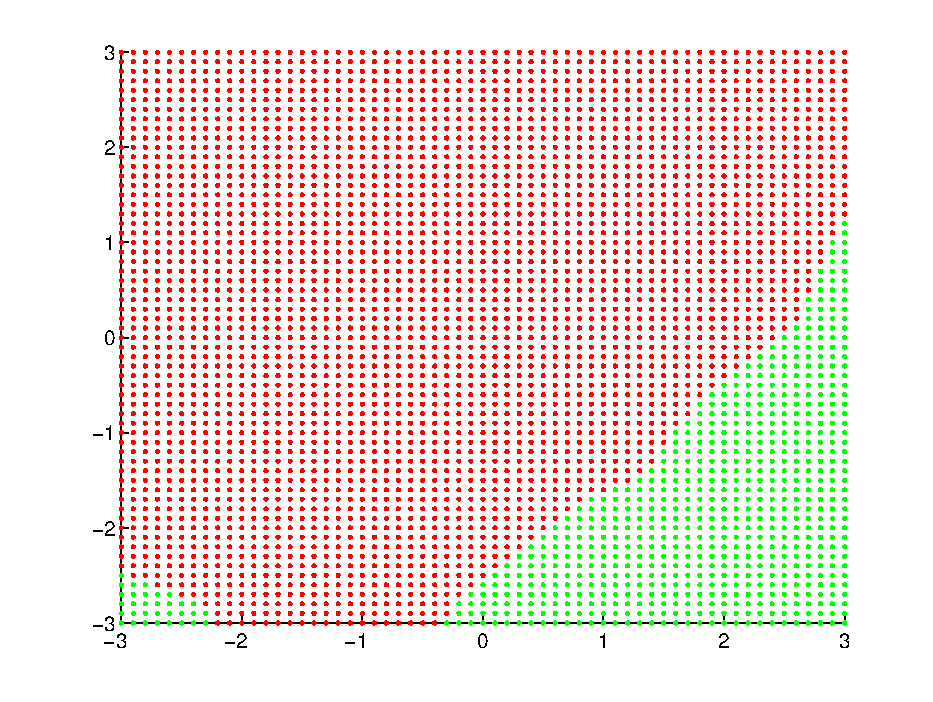
\includegraphics[width=0.6\textwidth]{./images/q209.pdf}
  \caption{The prediction trend when the loss matrix is used. Red dots are cancer predictions; green are healthy.}
  \label{fig:q29}
\end{figure}
